% Round-3 data figure, generated by export_eab3.py (figures/fig-planning.pdf).
\begin{figure}[t]
\centering
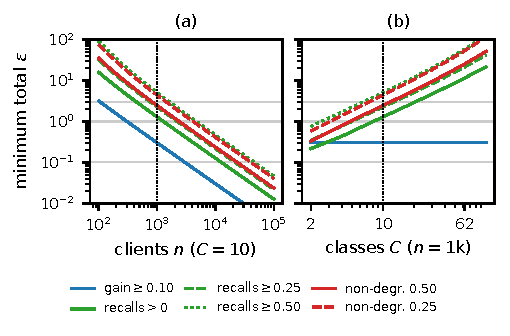
\includegraphics[width=\columnwidth]{figures/fig-planning.pdf}
\Description{Minimum total privacy budget of each publication target as a
function of the number of clients and of classes.}
\caption{Verification planning map (Gaussian approximation of the acceptance probability; given effect sizes, no further private query; the plotted effect sizes come from recorded private candidates). Minimum
total $\varepsilon$ at which each target of Table~\ref{tab:verify-ladder} is
accepted with probability $1/2$ under the fixed $50/25/25$ split, at the
median effect sizes of the recorded candidates. (a) $C=10$; (b) $n=1$k.
Dotted lines: the tested setting; grey lines: the tested budgets.}
\label{fig:planning}
\end{figure}
